\documentclass[tikz,border=3pt]{standalone}
\usepackage[T1]{fontenc}
\usepackage{amsmath}\usepackage{graphicx}
\usepackage{XCharter}
\usepackage[xcharter]{newtxmath}
\usepackage[scaled=.92]{helvet}
\usepackage{pgfplots}
\usetikzlibrary{arrows.meta,positioning,fit,calc,backgrounds,decorations.pathreplacing,patterns}
\usepgfplotslibrary{groupplots,fillbetween}
\pgfplotsset{compat=1.18}
\definecolor{ink}{HTML}{172536}
\definecolor{rgb}{HTML}{3563B8}
\definecolor{event}{HTML}{17857C}
\definecolor{fusion}{HTML}{76529C}
\definecolor{reference}{HTML}{8994A3}
\definecolor{warn}{HTML}{AC5948}
\definecolor{muted}{HTML}{657183}
\definecolor{rule}{HTML}{D9E0E8}
\definecolor{pale}{HTML}{F5F7FA}
\color{ink}
\tikzset{box/.style={rounded corners=2pt,draw=rule,fill=white,align=center,inner sep=4pt,font=\sffamily\fontsize{9}{10.8}\selectfont,minimum height=9mm},rb/.style={box,draw=rgb!50,fill=rgb!5},eb/.style={box,draw=event!50,fill=event!5},fb/.style={box,draw=fusion!55,fill=fusion!5},arrow/.style={-{Latex[length=1.8mm]},line width=.65pt,draw=muted},note/.style={font=\sffamily\fontsize{8.4}{10.2}\selectfont,align=center,text=muted},heading/.style={font=\sffamily\fontsize{10}{12}\selectfont\bfseries,align=left,text=ink}}
\pgfplotsset{paper/.style={width=15.7cm,height=6cm,axis lines*=left,axis line style={rule},tick style={draw=none},tick label style={font=\sffamily\fontsize{8.8}{10.4}\selectfont,text=muted},label style={font=\sffamily\fontsize{9.4}{11}\selectfont,text=ink},title style={font=\sffamily\fontsize{10}{12}\selectfont\bfseries,text=ink},legend style={draw=none,fill=none,font=\sffamily\fontsize{9}{11}\selectfont,cells={anchor=west}},grid=major,grid style={rule!65,line width=.3pt},minor tick num=0,scaled ticks=false,unbounded coords=jump,clip mode=individual}}

\hyphenpenalty=10000\exhyphenpenalty=10000
\tikzset{box/.append style={font=\sffamily\fontsize{8}{10}\selectfont},
note/.append style={font=\sffamily\fontsize{8}{10}\selectfont}}
% Generated by scripts/make_official_results.py; do not edit by hand.
\providecommand{\OfficialPhasePublishedOverallMiD}{35.80}
\providecommand{\OfficialOverallAbsoluteGain}{9.228548419}
\providecommand{\OfficialBandContributionSubtotal}{9.227548419}
\providecommand{\OfficialDisplayRoundingResidual}{0.0010}
\providecommand{\OfficialCrucialSmallContributionShare}{82.4\%}
\providecommand{\OfficialPhaseOverallMiD}{35.8015}
\providecommand{\OfficialGarlOverallMiD}{45.03}
\providecommand{\OfficialOverallRelativeGain}{20.49\%}
\providecommand{\OfficialPhaseCrucialMiD}{43.5190}
\providecommand{\OfficialGarlCrucialMiD}{53.13}
\providecommand{\OfficialCrucialRelativeGain}{18.09\%}
\providecommand{\OfficialPhaseSmallMiD}{28.2568}
\providecommand{\OfficialGarlSmallMiD}{37.58}
\providecommand{\OfficialSmallRelativeGain}{24.81\%}
\providecommand{\OfficialPhaseLargeMiD}{25.7179}
\providecommand{\OfficialGarlLargeMiD}{40.61}
\providecommand{\OfficialLargeRelativeGain}{36.67\%}
\providecommand{\OfficialPhaseNegativeMiD}{29.9314}
\providecommand{\OfficialGarlNegativeMiD}{31.29}
\providecommand{\OfficialNegativeRelativeGain}{4.34\%}
\providecommand{\OfficialSampleCount}{6,762}
\providecommand{\OfficialPhaseFailureRate}{0.0\%}
\providecommand{\OfficialGarlFailureRate}{0.0\%}
\providecommand{\OfficialPhaseSubmissionID}{1016512}
\providecommand{\OfficialGarlSubmissionID}{817519}

\begin{document}

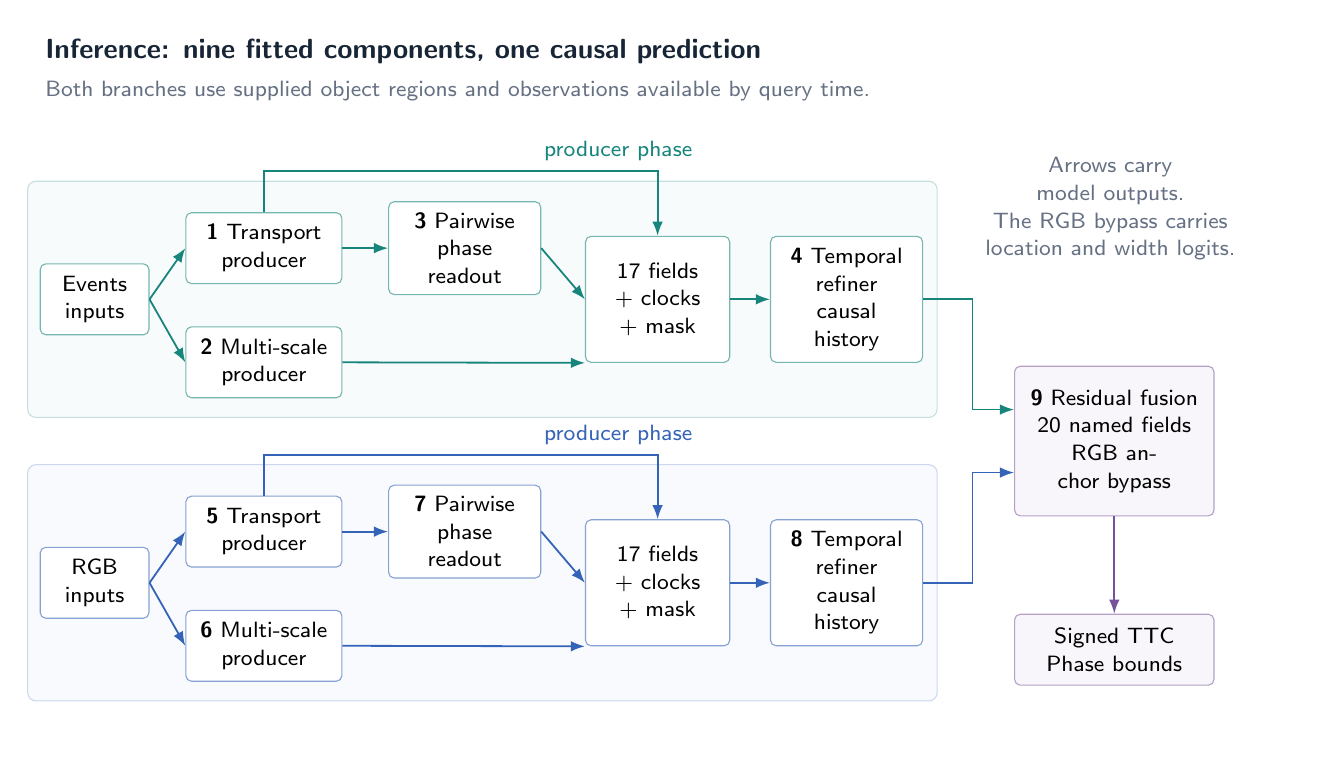
\begin{tikzpicture}[x=1cm,y=1cm]
\path[use as bounding box] (0,-.25) rectangle (16.2,8.8);
\node[heading,anchor=west] at (.1,8.5) {Inference: nine fitted components, one causal prediction};
\node[note,anchor=west] at (.1,8) {Both branches use supplied object regions and observations available by query time.};
\foreach \y/\col/\stream/\na/\nb/\np/\nc in {5.35/event/Events/1/2/3/4,1.75/rgb/RGB/5/6/7/8}{
 \draw[draw=\col!25,fill=\col!3,rounded corners=3pt] (0,\y-1.5) rectangle (11.55,\y+1.5);
 \node[box,draw=\col!60,text width=1.1cm] (in\na) at (.85,\y) {\stream\\inputs};
 \node[box,draw=\col!60,text width=1.7cm] (a\na) at (3,\y+.65) {\textbf{\na} Transport\\producer};
 \node[box,draw=\col!60,text width=1.7cm] (b\na) at (3,\y-.8) {\textbf{\nb} Multi-scale\\producer};
 \node[box,draw=\col!60,text width=1.65cm] (p\na) at (5.55,\y+.65) {\textbf{\np} Pairwise\\phase readout};
 \node[box,draw=\col!60,text width=1.55cm,minimum height=16mm] (f\na) at (8,\y) {17 fields\\+ clocks\\+ mask};
 \node[box,draw=\col!60,text width=1.65cm,minimum height=16mm] (c\na) at (10.4,\y) {\textbf{\nc} Temporal\\refiner\\causal history};
 \draw[arrow,\col] (in\na.east)--(a\na.west);
 \draw[arrow,\col] (in\na.east)--(b\na.west);
 \draw[arrow,\col] (a\na.east)--(p\na.west);
 \draw[arrow,\col] (p\na.east)--(f\na.west);
 \draw[arrow,\col] (b\na.east)--(f\na.south west);
 \draw[arrow,\col] (a\na.north)--++(0,.52)-|node[pos=.45,above,note,text=\col]{producer phase}(f\na.north);
 \draw[arrow,\col] (f\na.east)--(c\na.west);
}
\node[fb,text width=2.25cm,minimum height=19mm] (fusion) at (13.8,3.55) {\textbf{9} Residual fusion\\20 named fields\\RGB anchor bypass};
\draw[arrow,event] (c1.east)--(12,5.35)|-([yshift=4mm]fusion.west);
\draw[arrow,rgb] (c5.east)--(12,1.75)|-([yshift=-4mm]fusion.west);
\node[fb,text width=2.25cm] (out) at (13.8,.9) {Signed TTC\\Phase bounds};
\draw[arrow,fusion] (fusion.south)--(out.north);
\node[note,text width=3.3cm] at (13.75,6.5) {Arrows carry model outputs.\\The RGB bypass carries\\location and width logits.};
\end{tikzpicture}
\end{document}
